%   File: Crane.tex
% Author: Adam Leeper
%------------------------------------------------------------------------------
%\\[0.45pc]
\providecommand{\isolatedBuild}[1]{#1}% fallback definition lets this file build normally
\isolatedBuild{
  \documentclass[11pt,letterpaper]{article}
  %\documentclass[11pt,letterpaper]{book}

% aleeper: I think these are needed for Paul's macros?
\usepackage{epsfig}
\usepackage{epstopdf}

%\makeatletter
%\typeout{The import path is \import@path}
%\makeatother

\usepackage{import}

\subimport{./}{packagesMitiguy.sty}
\subimport{./}{macrosMitiguy.tex}
\subimport{./}{PageStylesMitiguy.tex}
\subimport{./}{macrosLeeper.tex}
 % Requires the TEXINPUTS environment variable.
  \isolatedBuildHeader
    {Velocity}
    {Velocity of a Wrecking Ball}
}
%%%
%%%
%%%
%------------------------------------------------------------------------------------------------
The figure shows a crane cab \basis{A} supporting a boom
\basis{B} that swings a wrecking ball $C_o$.
%
\Dextral ~orthogonal unit vectors (\uvecxyz{n}), (\uvecxyz{b}),
and (\uvecxyz{c}) are fixed in \basis{N}, \basis{B}, and \basis{C} respectively, as shown.
%
%
\\[0.45pc]
\begin{minipage}[t]{0.52\linewidth}
  \vspace*{0pt}
  The position vector from $N_o$ to $C_o$ is
  $$\posvec{N_o}{C_o} \equals[\;] x~\uvecx{n} \plus[\;] L_B ~\uvecx{b}
                                 \minus[\;] L_C ~\uvecy{c}$$

  %\\[0.45pc]
  %The angular velocity of \basis{B} in \basis{N} is
  %$\angvel{B}{N} \equals[\;] \thetadot_B ~\uvecz{b}$.
  %\\[0.25pc] The angular velocity of \basis{C} in \basis{N} is
  %$\angvel{C}{N} \equals[\;] \thetadot_C ~\uvecz{c}$.
  %
  {\small
    \begin{tabular}{|l|c|c|}
              \hline Quantity & Symbol & Type
      \\[0.0pc] \hline \uvecx{b} distance between $A_B$ and $B_C$
                & $L_B$ & Constant
      \\[0.0pc]        \uvecy{c} distance between $B_C$ and $C_o$
                & $L_C$ & Constant
      \\[0.0pc] \hline \uvecx{n} distance between $N_o$ to $A_B$
                & $x$ & Variable
      \\[0.0pc]        angle between \uvecx{n} and \uvecx{b} about \uvecz{n}
                & $\theta_B$ & Variable
      \\[0.0pc]        angle between \uvecy{n} and \uvecy{c} about \uvecz{n}
                & $\theta_C$ & Variable
      \\[0.0pc]\hline
    \end{tabular}
  }
\end{minipage}
\hfill
\begin{minipage}[t]{0.45\linewidth}
  \vspace*{0pt}
  \flushright
  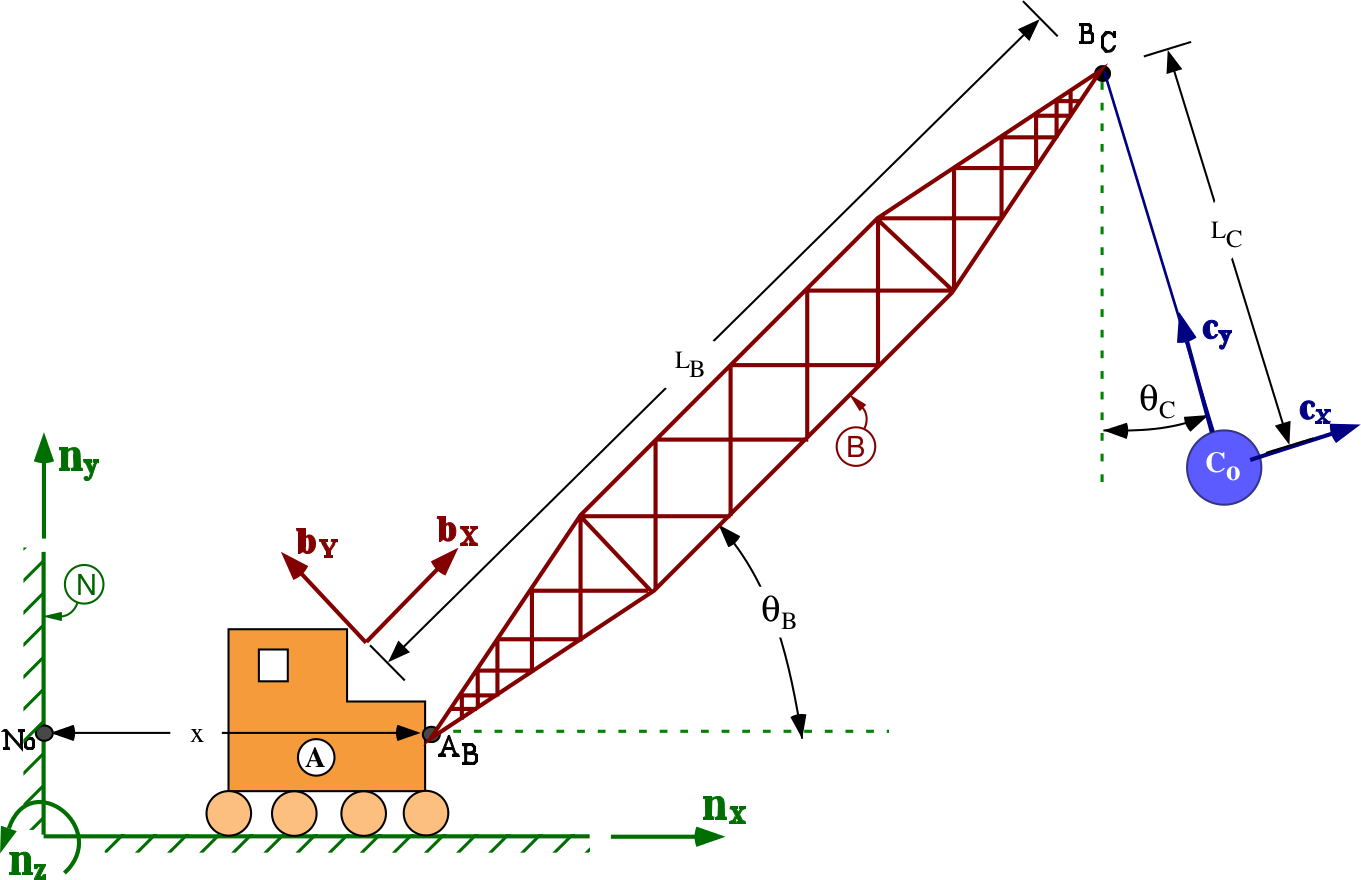
\includegraphics[width=0.99\linewidth]{crane_transparent.png}
\end{minipage}
%
%
%
\begin{enumerate}
  \item Determine:
    \\[0.0pc]
    \begin{tabular}{@{~$\bullet$~~}l}
        the angular velocity of \basis{B} in \basis{N}
        (or, \basis{B}'s angular velocity in \basis{N}).
      \\[0.0pc]
        the angular velocity of \basis{C} in \basis{N}
        (or, \basis{C}'s angular velocity in \basis{N}).
      \\[0.0pc]
        the angular velocity of \basis{C} in \basis{B}
        (or, \basis{C}'s angular velocity in \basis{B}).
    \end{tabular}
    \\[0.0pc]
    \Solution {}{1.0\linewidth}{
      The first two are ``simple'' rotations (see section 7.3.3),
      so angular velocity is formed \textbf{by inspection}.
      For example, imagine $\theta_B$ is zero, and align your (right-hand!)
      fingers with $\uvecx{b} \equals[\;] \uvecx{n}$.
      Then mentally increase $\theta_B$ and curl your fingers in the direction
      of rotation.
      Your thumb gives the direction vector associated with \angvel{B}{N}.
      \\[0.45pc]
      \begin{tabular}{ll}
        $\angvel{B}{N} \equals[\;] \thetadot_B ~\uvecz{n}$
        &
        \hspace{1cm}$\angvel{C}{N} \equals[\;] \thetadot_C ~\uvecz{n}$
      \end{tabular}
      \\[0.45pc]
      For \angvel{C}{B} it is easiest to use the angular velocity
      addition theorem (see section 7.3.4 - 7.3.5).
      \\[0.55pc]
      \begin{tabular}{l}
        $\angvel{C}{B} \equals[\;] \angvel{N}{B} + \angvel{C}{N}
                       \equals[\;] (-\thetadot_B + \thetadot_C) ~\uvecz{n}$
      \end{tabular}
      \\[0.0pc]
    }
    %
  \item Compute the velocity of $C_o$ in \basis{N} in terms of symbols
        in the table and their time derivatives.
    \\[0.45pc]
    %
    \begin{tabular}{@{}l@{}c@{}l}
      $\vel{C_o}{N}$ & $\equals[\;]$ & $\hidemath{
      \xdot~\uvecx{n} \plus[\;] L_B \thetadot_B \uvecy{b}
                      \plus[\;] L_C \thetadot_C \uvecx{c}}$
    \end{tabular}
    \\[0.45pc]
    \Solution {}{1.0\linewidth}{
      \begin{tabular}{@{}l@{~}c@{~}l}
      $\vel{C_o}{N}$ & $\deff[\;]$ & $\dt[N]{}~\posvec{N_o}{C_o}$
      $\equals[\;]$  $\dt[N]{}(x~\uvecx{n} \plus[\;] L_B ~\uvecx{b}
                   \minus[\;] L_C ~\uvecy{c})$
      \end{tabular}
      \\[0.45pc]
      We distribute first to get separate chunks to which we can then
      apply the golden rule:
      \\[0.45pc]
%      \hspace*{0.7cm}
      \begin{tabular}{@{}l@{~}c@{~}c@{}c@{}c@{}c@{}c}
        $\phantom{\vel{C_o}{N}}$ & \equals[\;] &
        $\dt[N]{}(x~\uvecx{n})$ & $\plus[\;]$ & $\dt[N]{}(L_B ~\uvecx{b})$
        & $\minus[\;]$ & $\dt[N]{}(L_C ~\uvecy{c})$
      \\[0.45pc]
        & \equals[\;] &
        $\dt[N]{}(x~\uvecx{n})$ &
        $\plus[\;]$ & $[~\dt[B]{}(L_B ~\uvecx{b}) + \angvel{B}{N}
         \times (L_B ~\uvecx{b}) ~]$ &
        $\minus[\;]$ & $[~\dt[C]{}(L_C ~\uvecy{c}) + \angvel{C}{N}
         \times (L_C ~\uvecy{c})~]$
      \\[0.45pc]
        & \equals[\;] &
        $\dt[N]{}(x~\uvecx{n})$ &
        $\plus[\;]$ & $[~\dt[B]{}(L_B ~\uvecx{b}) +
         (\thetadot_B ~\uvecz{n}) \times (L_B ~\uvecx{b}) ~]$ &
        $\minus[\;]$ & $[~\dt[C]{}(L_C ~\uvecy{c}) +
         (\thetadot_C ~\uvecz{n}) \times (L_C ~\uvecy{c})~]$
      \\[0.45pc]
        & \equals[\;] &
        $\xdot~\uvecx{n}$ &
        $\plus[\;]$ & $[~0 + L_B \thetadot_B (\uvecy{b})~]$ &
        $\minus[\;]$ & $[~0 + L_C \thetadot_C (-\uvecx{c})~]$
      \\[0.45pc]
        & \equals[\;] &
        $\xdot~\uvecx{n}$ &
        $\plus[\;]$ & $L_B \thetadot_B \uvecy{b}$ &
        $\plus[\;]$ & $L_C \thetadot_C \uvecx{c}$
      \end{tabular}
      \\[0.45pc]
      \textbf{Intuition Check}
      \\[0.45pc]
      Take a moment to mentally visualize the movement of $C_o$ caused by
      each ``degree-of-freedom" (loosely speaking: each variable),
      and check that the terms of \vel{C_o}{N} seem to describe that motion.
      \\[0.45pc]
      \textbf{Checking Consistency of the Result}
      \\[0.45pc]
      Vectors (like anything) must have the same units in order to
      add, so this is an easy way to check the result.
      It's a velocity, so each term must have the
      dimensions of length per time. In SI units, the first term is
      $\frac{m}{s}$ and the second and third terms are $m*\frac{rad}{s}$,
      which is equivalent to $\frac{m}{s}$ since radians are ``unit-less".
    }
    %
    %
    \clearpage
  \item Compute the acceleration of $C_o$ in \basis{N}.
    %(It is probably easiest to just differentiate your result from (a),
    %but
    %\\[0.0pc]
    If it helps, you can use $\accel{Bc}{N} = \ddot{x}~\uvecx{n}
    + L_B \thetaddot_B ~\uvecy{b} - L_B (\thetadot_B)^2 ~\uvecx{b}$.
    \\[0.45pc]
    \begin{tabular}{@{}l@{}c@{}l}
      $\accel{C_o}{N}$ & $\equals[\;]$
      & $\hidemath{\xddot~\uvecx{n} \plus[\;] L_B \thetaddot_B ~\uvecy{b}
                   \minus[\;] L_B (\thetadot_B)^2 ~\uvecx{b}
                   \plus[\;] L_C \thetaddot_C ~\uvecx{c}
                   \plus[\;] L_C (\thetadot_C)^2 ~\uvecy{c}}$
    \end{tabular}
    \\[0.45pc]
    % and observe that $B_C$ and $C_o$ are both fixed in \basis{C}.)
    %\\[0.45pc] $\accel{C_o}{N} \equals[\;]$
    %\\[11.0pc]
    \Solution {}{1.0\linewidth}{
      \textbf{Solution 1: Differentiation of Velocity}
      \\[0.45pc]
      Differentiating the result from the previous part:
      \\[0.45pc]
      \begin{tabular}{l@{}c@{}l}
        $\accel{\origin{C}}{N}$ & $\deff[\;]$ & $\dt[N]{}\vel{C_o}{N}$
       \\[0.45pc]
       &
        $\equals[\;]$ &
        $\dt[N]{}(\xdot~\uvecx{n} \plus[\;]
                  L_B \thetadot_B~\uvecy{b} \plus[\;]
                  L_C \thetadot_C~\uvecx{c})$
      \end{tabular}
      \\[-1.0pc]
      \begin{tabular}{l@{}c@{}c@{}c@{}c@{}c@{}c}
        $\phantom{\accel{\origin{C}}{N}}$
       \\[0.45pc]
        & $\equals[\;]$
        & $\dt[N]{}(\xdot~\uvecx{n})$
        & $\plus[\;]$
        & $\dt[N]{}(L_B \thetadot_B~\uvecy{b})$
        & $\plus[\;]$
        & $\dt[N]{}(L_C \thetadot_C~\uvecx{c})$
       \\[0.45pc]
        & $\equals[\;]$
        & $\dt[N]{}(\xdot~\uvecx{n})$
        & $\plus[\;]$
        & $[~\dt[B]{}(L_B \thetadot_B~\uvecy{b})
           \plus[\;] \angvel{B}{N} \CrossProduct
                   (L_B \thetadot_B~\uvecy{b})~]$
        & $\plus[\;]$
        & $[~\dt[c]{}(L_C \thetadot_C~\uvecx{c})
           \plus[\;] \angvel{C}{N} \CrossProduct
                   (L_C \thetadot_C~\uvecx{c})~]$
       \\[0.45pc]
        & $\equals[\;]$
        & $\dt[N]{}(\xdot~\uvecx{n})$
        & $\plus[\;]$
        & $[~\dt[B]{}(L_B \thetadot_B~\uvecy{b})
           \plus[\;] \angvel{B}{N} \CrossProduct
                   (L_B \thetadot_B~\uvecy{b})~]$
        & $\plus[\;]$
        & $[~\dt[c]{}(L_C \thetadot_C~\uvecx{c})
           \plus[\;] \angvel{C}{N} \CrossProduct
                   (L_C \thetadot_C~\uvecx{c})~]$
       \\[0.45pc]
        & $\equals[\;]$
        & $\ddot{x}~\uvecx{n}$
        & $\plus[\;]$
        & $L_B \thetaddot_B ~\uvecy{b}
            \minus[\;] L_B (\thetadot_B)^2 ~\uvecx{b}$
        & $\plus[\;]$
        & $L_C \thetaddot_C ~\uvecx{c}
            \plus[\;] L_C (\thetadot_C)^2 ~\uvecy{c}$
      \end{tabular}
      %
      \\[0.45pc]
      \textbf{Solution 2: Using Formulas for Two Points Fixed in a Rigid Frame}
      \\[0.45pc]
      Since $B_C$ and $C_o$ are both \textbf{fixed} in frame \basis{C},
      we can use the formulas from Mitiguy section 8.2.
      %
      Verify that you understand how the general formula was adapted
      to the specific frames and points in \textbf{this} problem to obtain
      the equation below.
      \\[0.45pc]
      \begin{tabular}{l}
        $\accel{C_o}{N} = \accel{B_c}{N}
        \plus[\;] \alf{C}{N} \CrossProduct \posvec{B_C}{C_o}
        \plus[\;] \angvel{C}{N} \CrossProduct
        (\angvel{C}{N} \CrossProduct \posvec{B_C}{C_o})$
      \end{tabular}
      \\[0.45pc]
      We'll form each term separately:
      \\[0.0pc]
      \parbox{1.0\linewidth}{
      \begin{itemize}
        \item The first term (\accel{B_c}{N}) was given.
        \item For the second term we need
              $\alf{C}{N} ~\deff~ \dt[N]{}\angvel{C}{N}
                          \equals[\;] \thetaddot_C ~\uvecz{n}$,
              so then we can calculate:
              \\[0.45pc]
              \begin{tabular}{l}
                $\alf{C}{N} \times \posvec{B_C}{C_o}
                \equals[\;] \thetaddot_C ~\uvecz{n} \times (-L_C \uvecy{c})
                \equals[\;] L_C \thetaddot_C ~\uvecx{c}$
              \end{tabular}
        \item The third term is:
              \\[0.45pc]
              \begin{tabular}{l@{$\equals[\;]$}l}
                  $\angvel{C}{N} \times
                  (\angvel{C}{N} \times \posvec{B_C}{C_o})$ &
                  $\thetadot_C ~\uvecz{n} \times
                  (\thetadot_C ~\uvecz{n} \times (-L_C \uvecy{c}))$
                  \equals[\;] $\thetadot_C ~\uvecz{n} \times
                      (L_C \thetadot_C ~\uvecx{c})$
                  \equals[\;] $L_C (\thetadot_C)^2 ~\uvecy{c}$
              \end{tabular}
      \end{itemize}
      }
      %
      Putting all the pieces together we have:
      \\[0.45pc]
      \begin{tabular}{l}
        $\accel{C_o}{N} \equals[\;]
          \ddot{x}~\uvecx{n}
          \plus[\;] L_B \thetaddot_B ~\uvecy{b} \minus[\;]
                    L_B (\thetadot_B)^2 ~\uvecx{b}
          \plus[\;] L_C \thetaddot_C ~\uvecx{c} \plus[\;]
                    L_C (\thetadot_C)^2 ~\uvecy{c}$
      \end{tabular}
      \\[1.0pc]
      \textbf{Checking Consistency of the Result}
      \\[0.45pc]
      Vectors (like anything) must have the same units in order to
      add, so this is an easy way to check the result.
      \parbox{1.0\linewidth}{
      \begin{itemize}
        \item $\xddot = \dt{}(\dt{}x)$ has dimensions of ((length/time)/time).
              In SI units, that would be $m/s^2$.
        \item $L_B$ and $L_C$ are both lengths (m), and $\thetaddot_B$ and
              $\thetaddot_C$ are both the second derivative of an angle
              ($\mathrm{rad}/s^2$).
              Radians are ``unit-less'', so $L_B \thetaddot_B$ and
              $L_C \thetaddot_C$ both have units of $m/s^2$.
        \item $\thetadot_B$ and $\thetadot_C$ are
              first derivatives of an angle (rad/s), so the units on $L_B
              (\thetadot_B)^2$ and $L_C (\thetadot_C)^2$ are both $m/s^2$.
      \end{itemize}
      \vspace{0.5pc}
      Finally, let's identify each term (see section 8.5) and check that
      it is consistent with the picture.
      \begin{itemize}
        \item The first term says that changes in $x$ cause $C_o$ to
              accelerate in the \uvecx{n} direction.
        \item The second term says there is an acceleration ``tangent''
              to the rotation described by $\theta_B$.
              %That is, it is caused by $\alf{B}{N}$, or the
              %second-derivative of $\theta_B$.
        \item The third term is due to the first-derivative of $\theta_B$
              (i.e. due to \basis{B}'s angular velocity in \basis{N}).
              Notice that it acts ``inward" toward the source of the
              rotation; this is a ``centripetal'' term.
        \item The fourth term says there is an acceleration ``tangent''
              to the rotation described by $\theta_C$.
              %That is, it is caused by $\alf{C}{N}$, or the
              %second-derivative of $\theta_C$.
        \item The fifth term is due to the first-derivative of
              $\theta_C$ (i.e. due to \basis{C}'s angular velocity in
              \basis{N}). Notice that it acts ``inward" toward the source
              of the rotation; this is another ``centripetal'' term.
      \end{itemize}
      }
    }  % end solution
\end{enumerate}

\isolatedBuildFooter
